\documentclass[a4paper,12pt]{extarticle}

\usepackage[T1]{fontenc}
\usepackage[utf8]{inputenc}
\usepackage{lmodern}

\usepackage[]{parskip}
\usepackage{hyperref, wrapfig, float, amsmath, adjustbox, array, pdflscape, soul, color, extsizes}
\usepackage{booktabs}
\usepackage{lscape}

\renewcommand{\arraystretch}{2}
\renewcommand{\contentsname}{Spis treści}
\renewcommand{\refname}{Bibliografia}
\renewcommand{\figurename}{Rys.}
\renewcommand{\tablename}{Tab.}

\usepackage{geometry}
\geometry{
  a4paper,
  margin=30mm,
  bottom=30mm
}

\usepackage{graphicx}
\usepackage[font=footnotesize,labelfont=bf,justification=centering]{caption}
\usepackage{subcaption}
\graphicspath{ {./images/}{../images/} }

\newcommand{\mathcolorbox}[1]{
  \begin{center}
    \colorbox{yellow}{$\displaystyle #1$}
  \end{center}
}
\newcommand{\pvec}[1]{
  \vec{#1}\mkern2mu\vphantom{#1}
}
\newcommand{\angstrom}{\mbox{\normalfont\AA}}

\begin{document}
  \begin{titlepage}
    \begin{center}
      \begin{figure}[H]
        \centering
        
\includegraphics[scale=.125]{logopp.png}
      \end{figure}
      \vspace*{.05\textheight}
      \huge\textbf{Politechnika Poznańska}\\
      \large\textbf{Wydział Inżynierii Materiałowej i Fizyki Technicznej}\\
      \large\textbf{Fizyka Techniczna}\\
      \vspace*{.2\textheight}
      \huge\textbf{Sprawozdanie --- laboratorium AFM}\\
      \vspace*{.025\textheight}
      \large\textbf{Jakub Bąbelek\\(nr.\ albumu: 136454)}
    \end{center}
  \end{titlepage}

  \tableofcontents
  
  \clearpage

  \section{Wstęp}
  Miskroskop sił atomowych --- AFM został skonstruowany w 1986 przez zespół:\\
  \textit{G.\ Binnig, C.\ F.\ Quate oraz Ch.\ Gerber}. Jest to rodzaj mikroskopu
  umożliwiający wykonywanie obrazu powierzchni z rozdzielczością atomową,
  wykorzystując siłę oddziaływań międzyatomowych.
  
  Ostrze --- umieszczone na sprężystej mikrobelce --- sunąc po lub bezpośrednio
  nad powierzchnią dostarcza informacji o sile oddziaływania międzyatomowego
  badanej powierzchni.

  \begin{figure}[H]
    \centering
    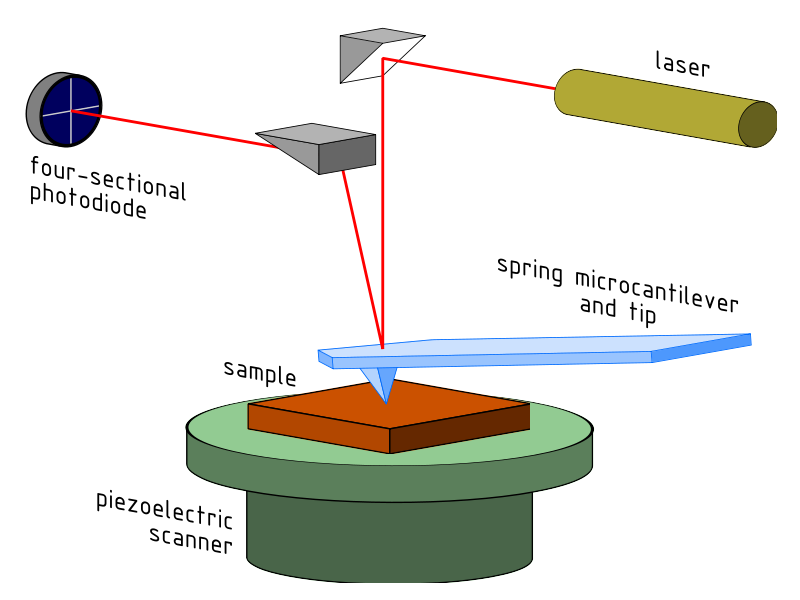
\includegraphics[width=10cm]{afm.png}
    \caption{Schemat budowy i zasada działania AFM}
    \label{fig:afm}
  \end{figure}

  Za pomocą mikroskopu sił atomowych można również dokonywać pomiarów sił tarcia,
  mierzy się wówczas skręcenie dźwignii. Do pomiaru odkształcenia wykorzystuje
  się metody optyczne (lub historycznie STM umieszczony ``na'' mikrobelce AFM)
  czułość takiej metody to wielkości rzędu dziesiątych części angstroma.

  W AFM do pomiarów możemy wykorzystać siły krótko i dalekozasięgowe, wyróżnić
  dzięki temu można następujące tryby pomiarowe:
  \begin{itemize}
    \item Tryb kontaktowy
    \item Tryb bezkontaktowy
    \item Tryb kontaktu przerywanego
  \end{itemize}

  Zebrane dane następnie poddaje się obróbce komputerowej np.\ w sposób jaki został
  przedstawiony w dalszej części sprawozdania.

  \clearpage

  \section{Topografia \( Au-SiO_x \)}

  Aby uzyskać obraz topografii poddałem dane obróbce w programie Gwyddion.
  Po użyciu funkcji \textit{Align rows} oraz usunięciu ``artefaktów'' obrazu
  objawiających się w formie poziomych ``cieni'' widocznych na obrazie topografii
  uzyskałem następujące obrazy.

  \begin{figure}[H]
    \centering
    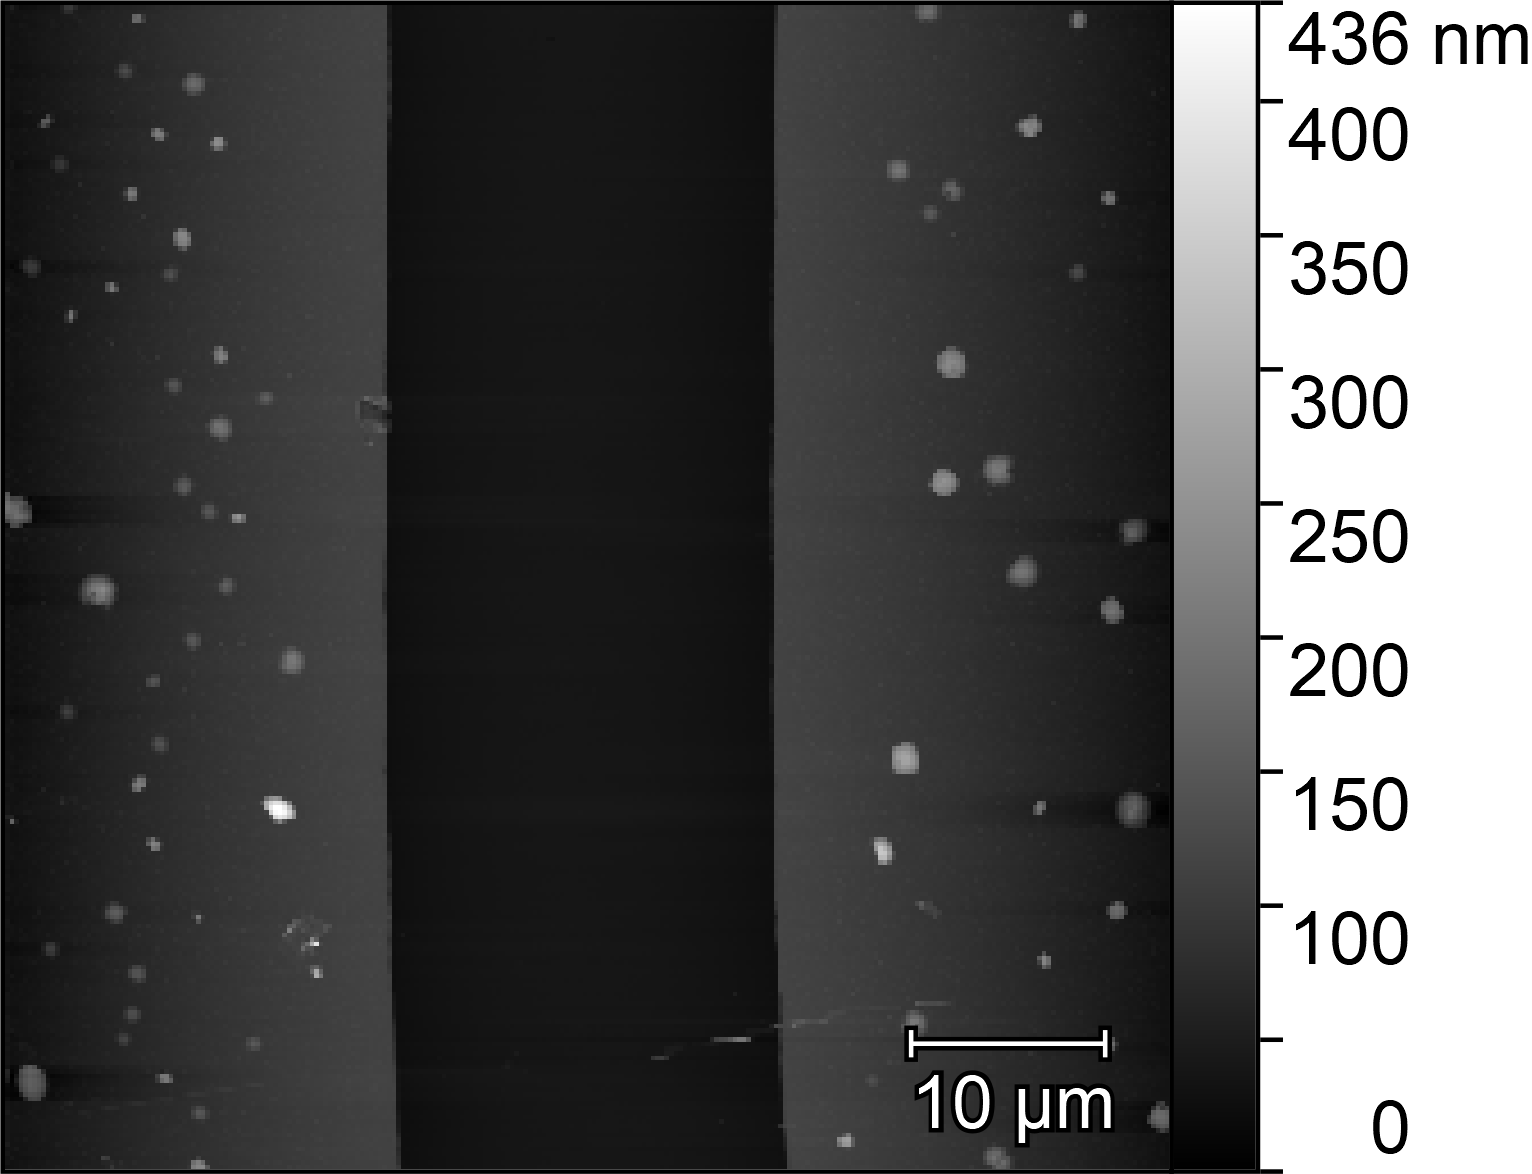
\includegraphics[width=10cm]{ausi_topo.png}
    \caption{Topografia po obróbce w programie Gwyddion}
    \label{fig:ausi_topo}
  \end{figure}

  Z obrazu przekroju (\figurename~\ref{fig:ausi_przekroj}) możemy odczytać
  szerokość paska tlenku krzemu która wynosi \(19.85\mu m\)

  \begin{figure}[H]
    \centering
    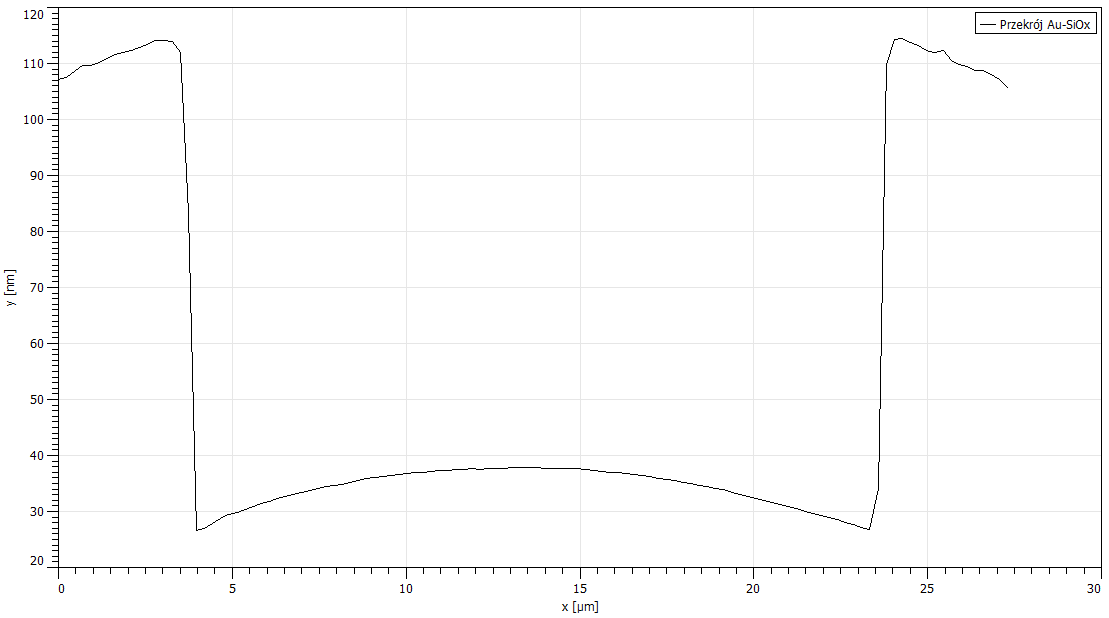
\includegraphics[width=10cm]{ausi_przekroj.png}
    \caption{Przekrój obrazu topografii}
    \label{fig:ausi_przekroj}
  \end{figure}
  \begin{figure}[H]
    \centering
    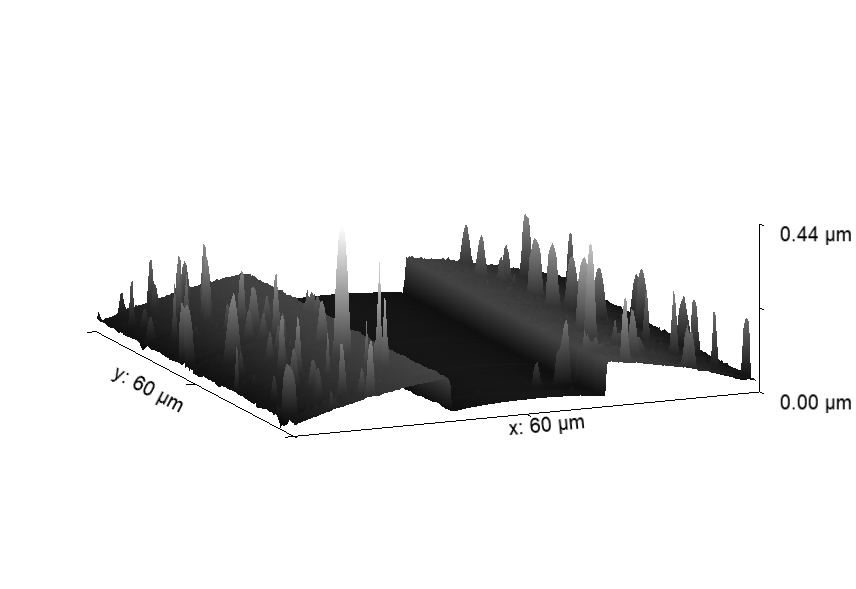
\includegraphics[width=10cm]{ausi_3d.png}
    \caption{Topografia --- widok 3d}
    \label{fig:ausi_3d}
  \end{figure}

  \section{Siatka kalibracyjna}

  Siatka kalibracyjna jest stosowana do kalibracji mikroskopów.

  \begin{figure}[H]
    \centering
    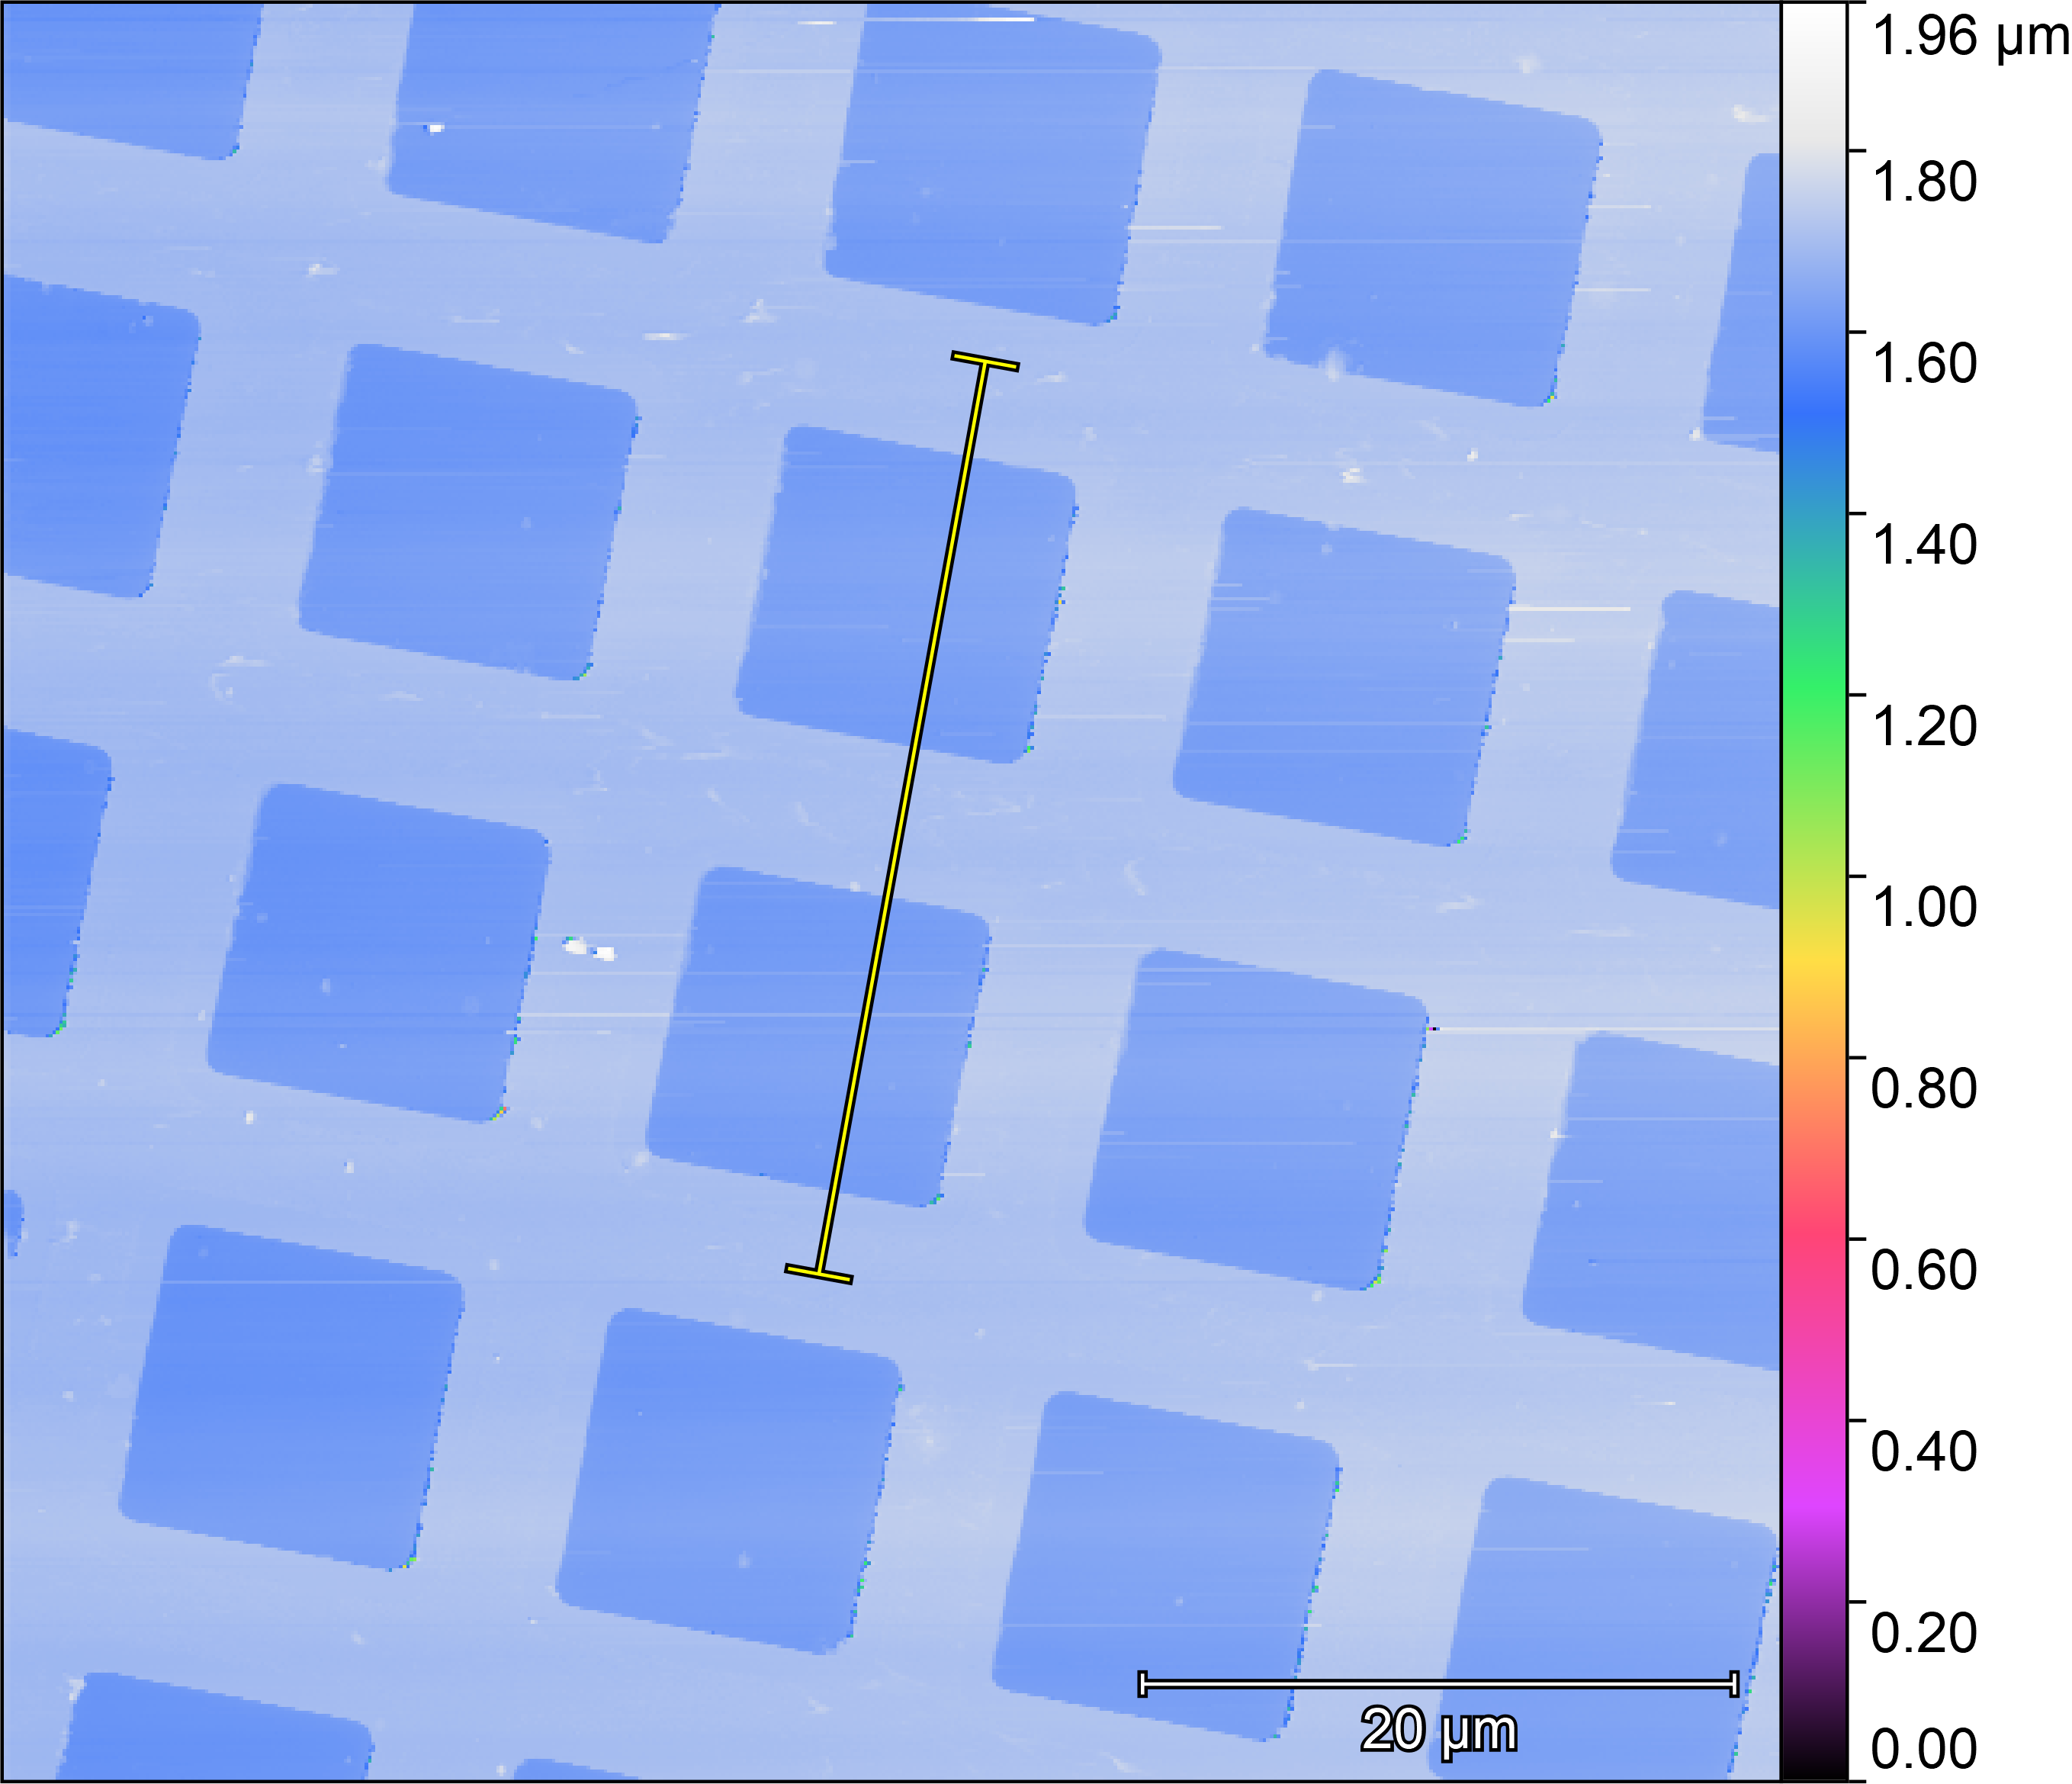
\includegraphics[width=10cm]{siatka_topo.png}
    \caption{Topografia siatki kalibracyjnej}
    \label{fig:siatka_topo}
  \end{figure}
  \begin{figure}[H]
    \centering
    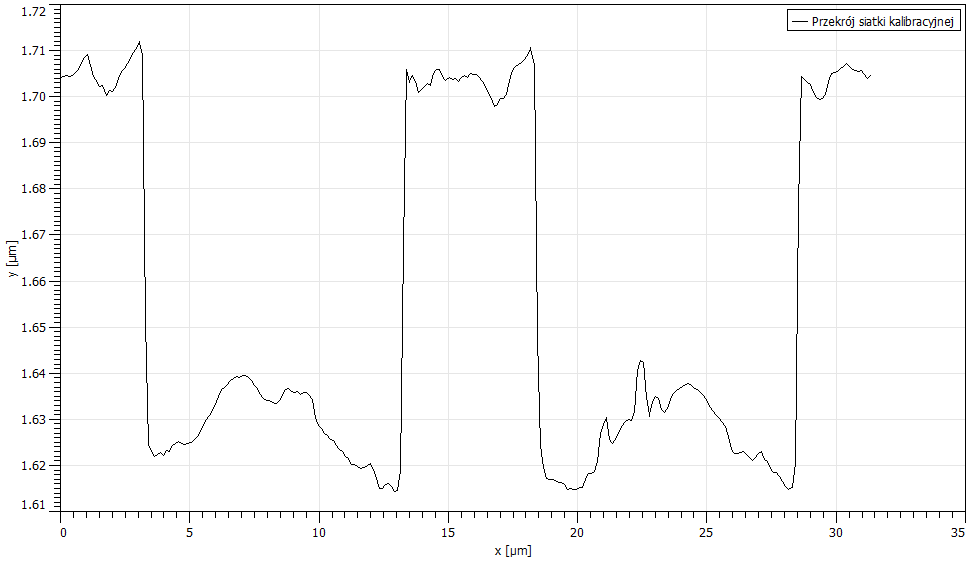
\includegraphics[width=10cm]{siatka_przekroj.png}
    \caption{Przekrój topografii siatki kalibracyjnej}
    \label{fig:siatka_przekroj}
  \end{figure}

  \section{Topografia matrycy CCD}
  \begin{figure}[H]
    \centering
    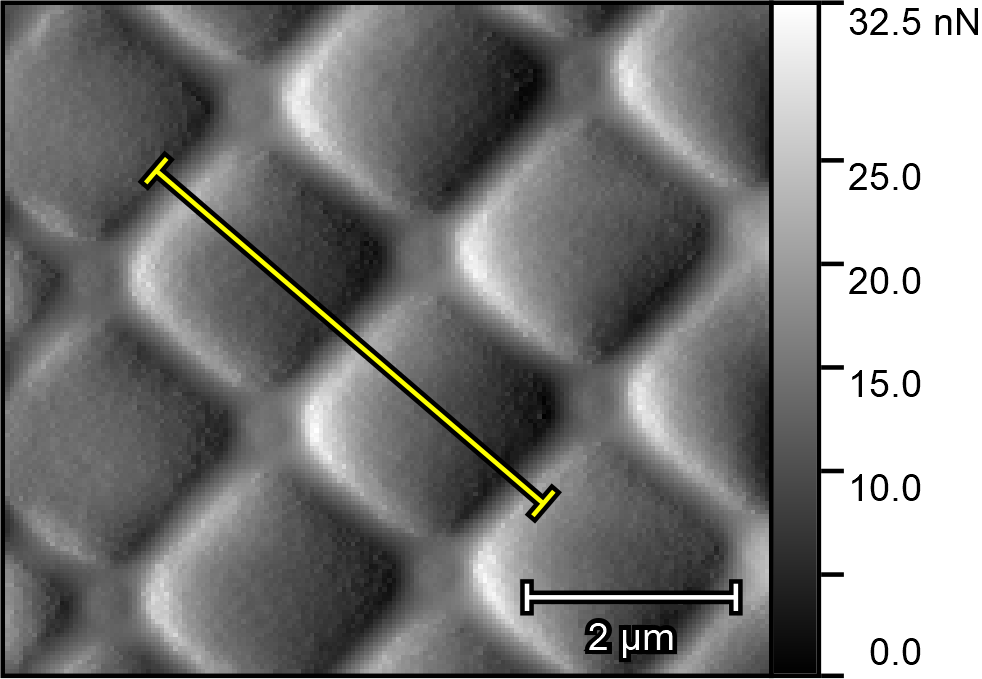
\includegraphics[width=10cm]{ccd_topo.png}
    \caption{Topografia matrycy CCD}
    \label{fig:ccd_topo}
  \end{figure}
  \begin{figure}[H]
    \centering
    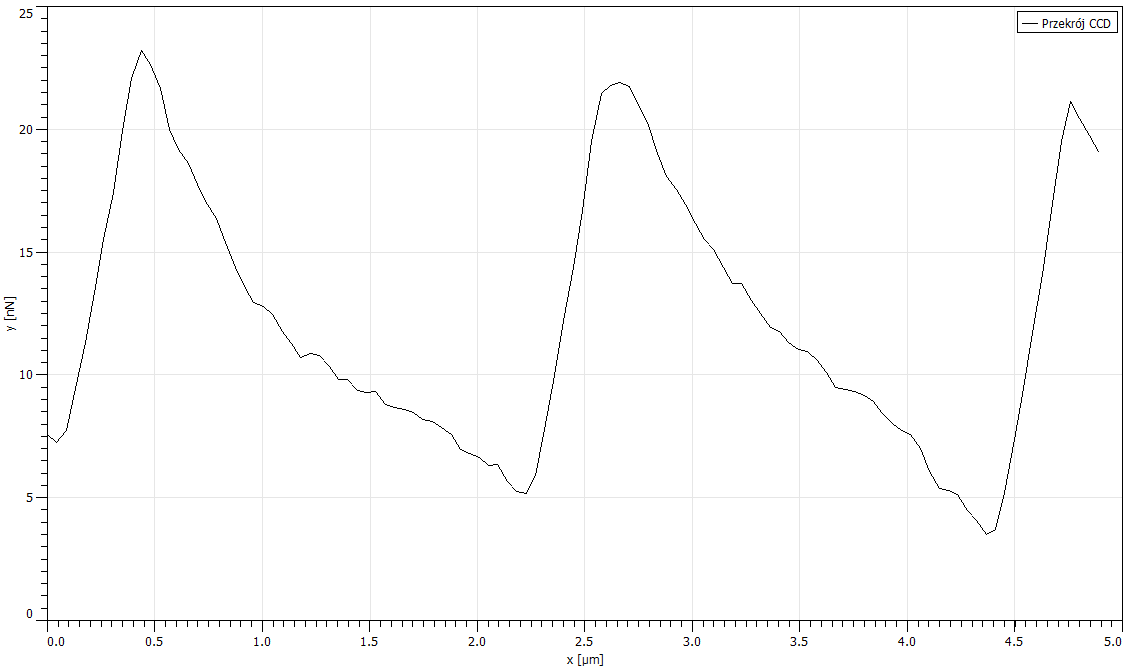
\includegraphics[width=10cm]{ccd_przekroj.png}
    \caption{Przekrój topografii matrycy CCD}
    \label{fig:ccd_przekroj}
  \end{figure}

  \section{Analiza płyt DVD oraz HD DVD}
  Ilość danych jakie możemy zapisać na płycie zależy od gęstości w jakiej znaleźć
  się one mogą na jej powierzchni, analiza danych z mikroskopu pozwala na obliczenie
  z jaką gęstością możliwy jest zapis na obu nośnikach.

  \subsection{DVD}

  \begin{figure}[H]
    \centering
    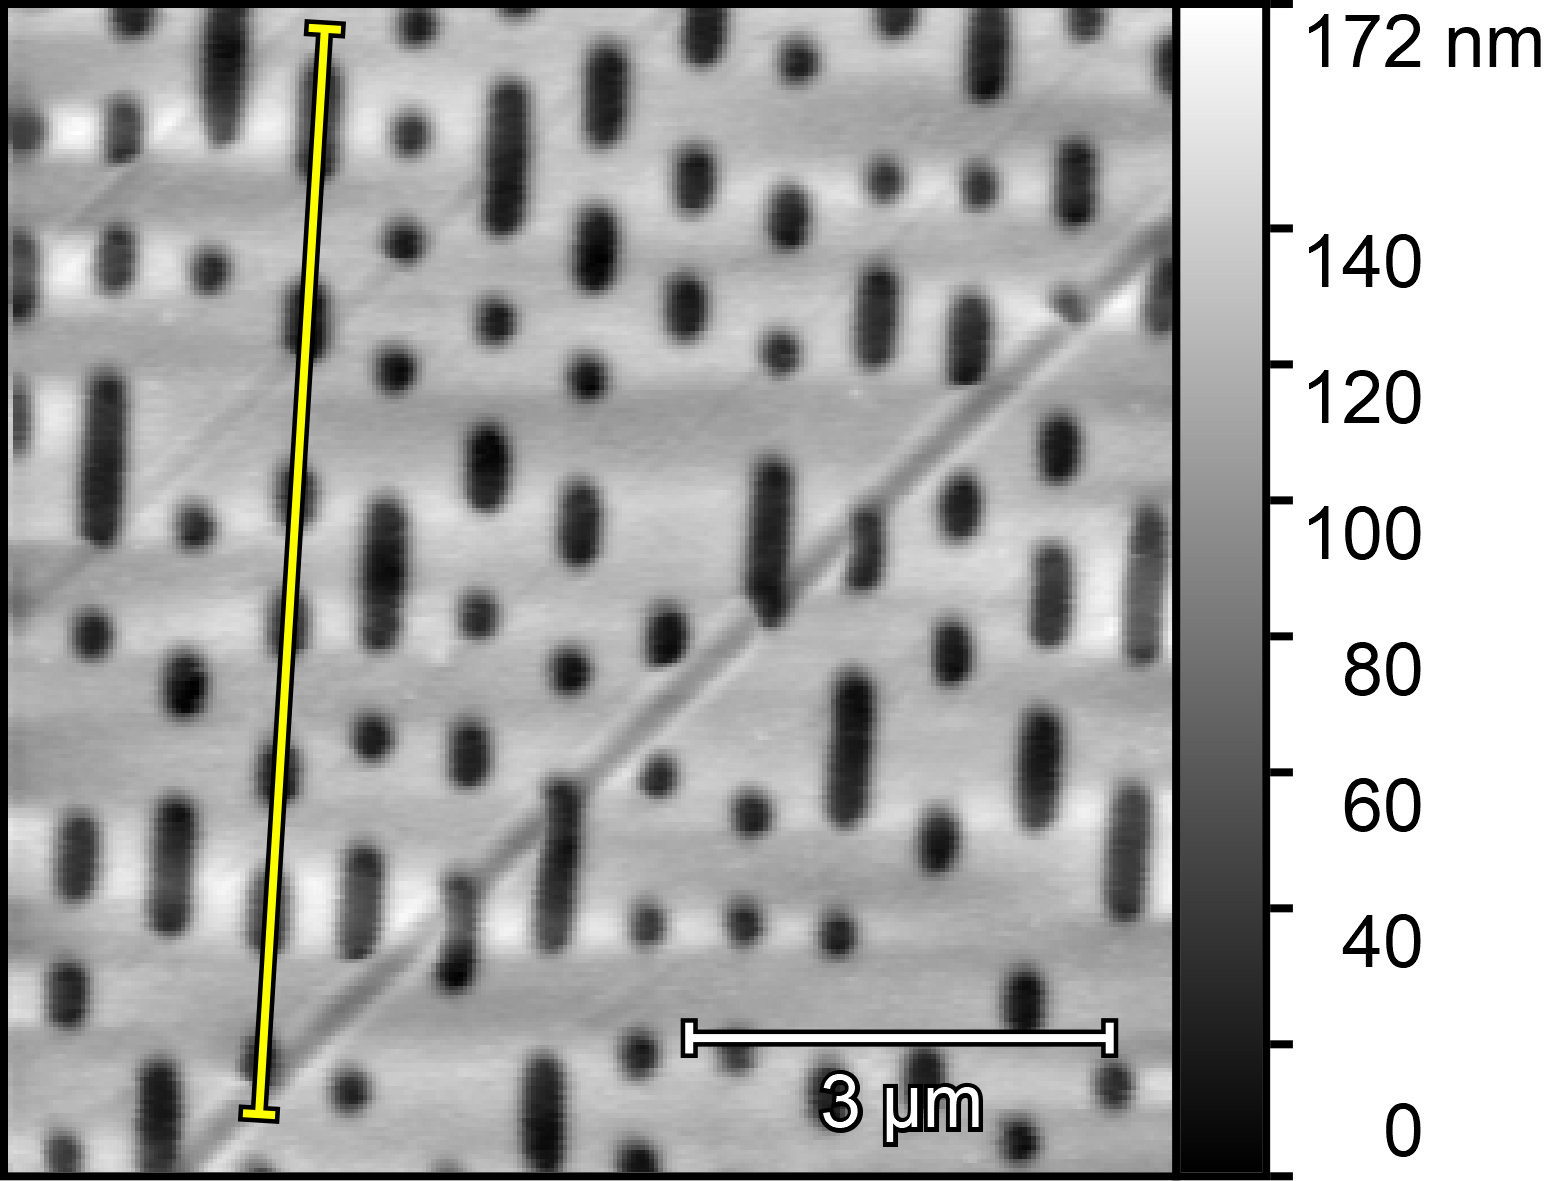
\includegraphics[width=10cm]{dvd_topo.png}
    \caption{Topografia płyty DVD}
    \label{fig:dvd_topo}
  \end{figure}

  \begin{figure}[H]
    \centering
    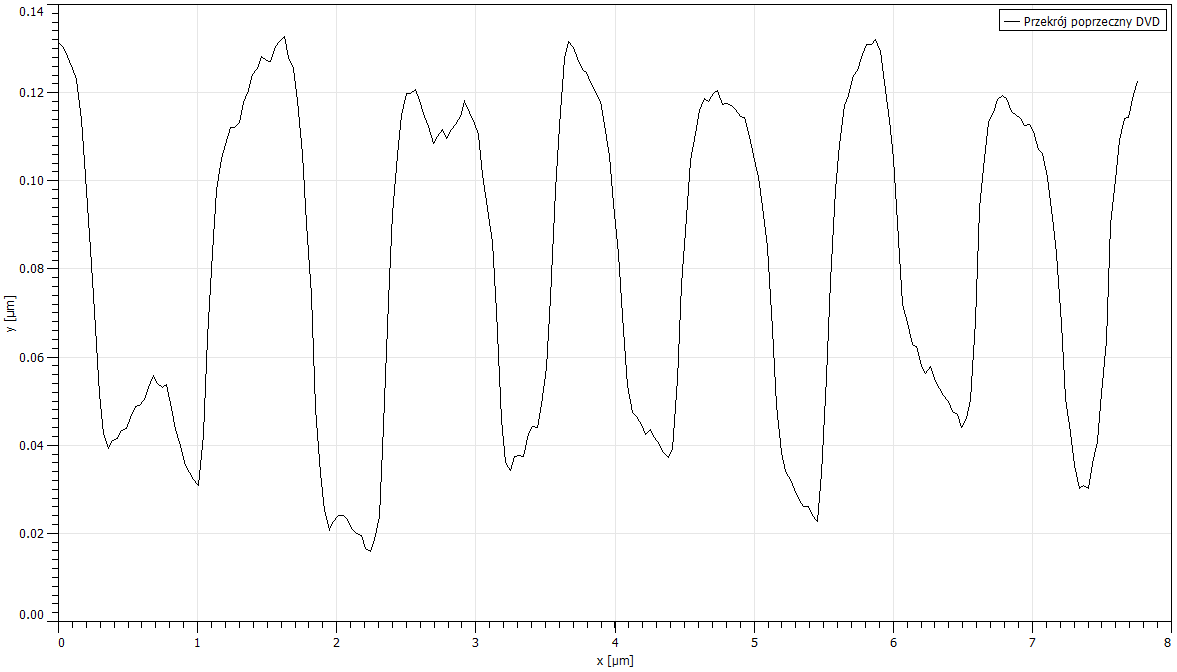
\includegraphics[width=10cm]{dvd_przekroj.png}
    \caption{Przekrój płyty DVD}
    \label{fig:dvd_przekroj}
  \end{figure}

  Zaznaczając maską wszystkie rowki (\figurename~\ref{fig:dvd_grains}) na
  płycie dvd i używając funkcji \textit{Grains summary} możemy policzyć ich
  ilość która wynosi 90

  \begin{figure}[H]
    \centering
    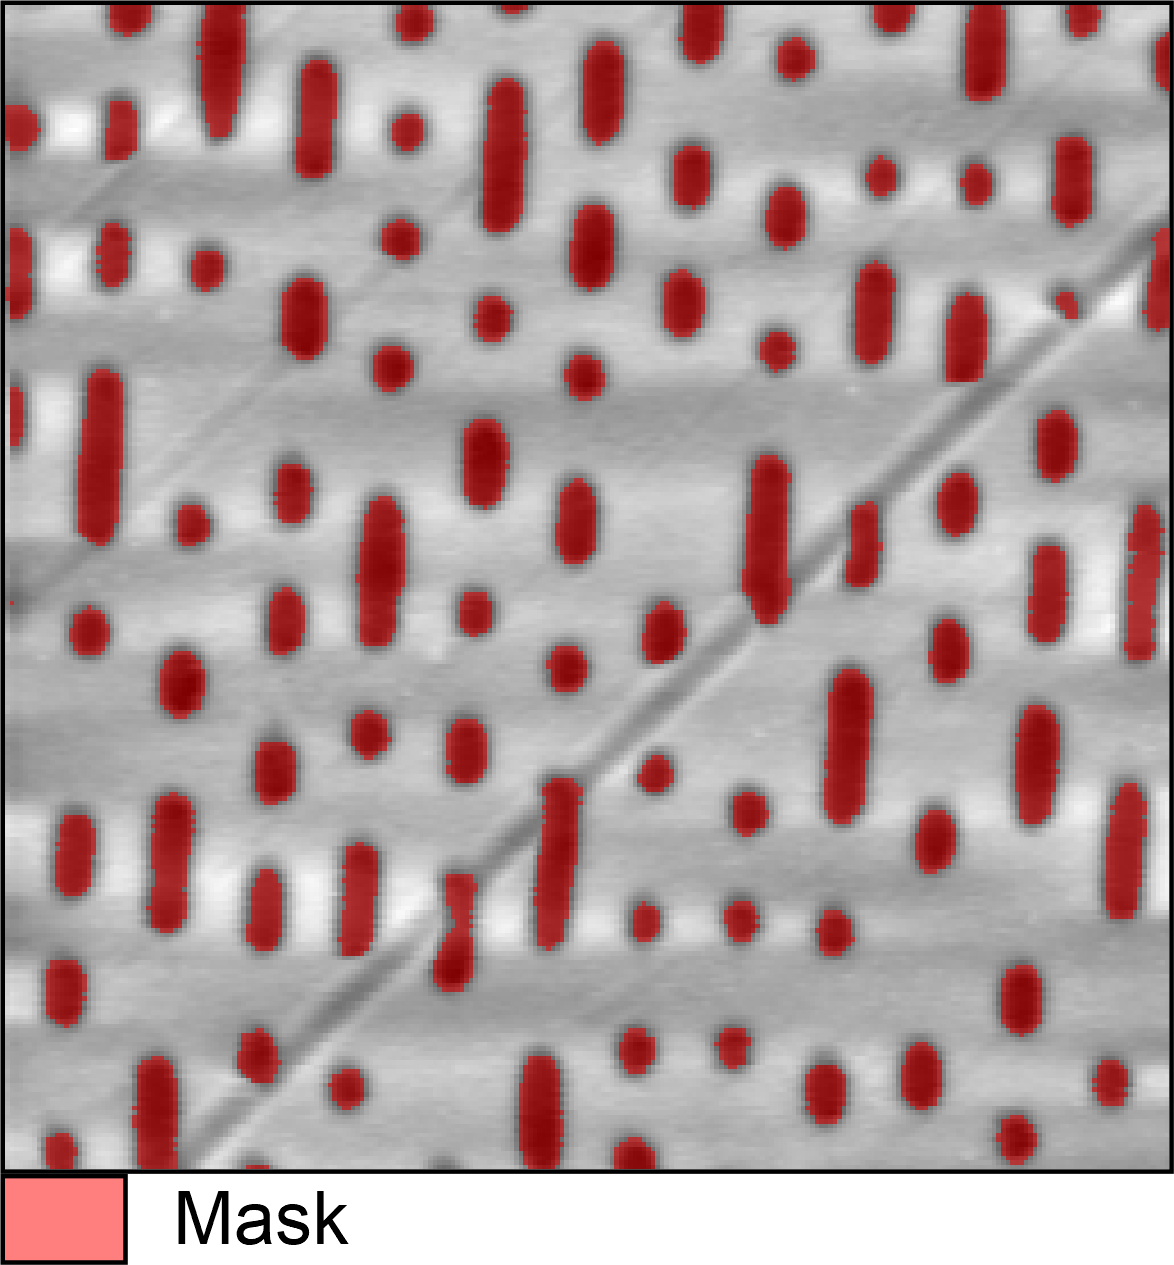
\includegraphics[width=7cm]{dvd_grains.png}
    \caption{Obraz po zaznaczeniu rowków dla płyty DVD}
    \label{fig:dvd_grains}
  \end{figure}

  \subsection{HD DVD}
  Wszystkie powyższe czynności zostały powtórzone dla płyty HD DVD

  \begin{figure}[H]
    \centering
    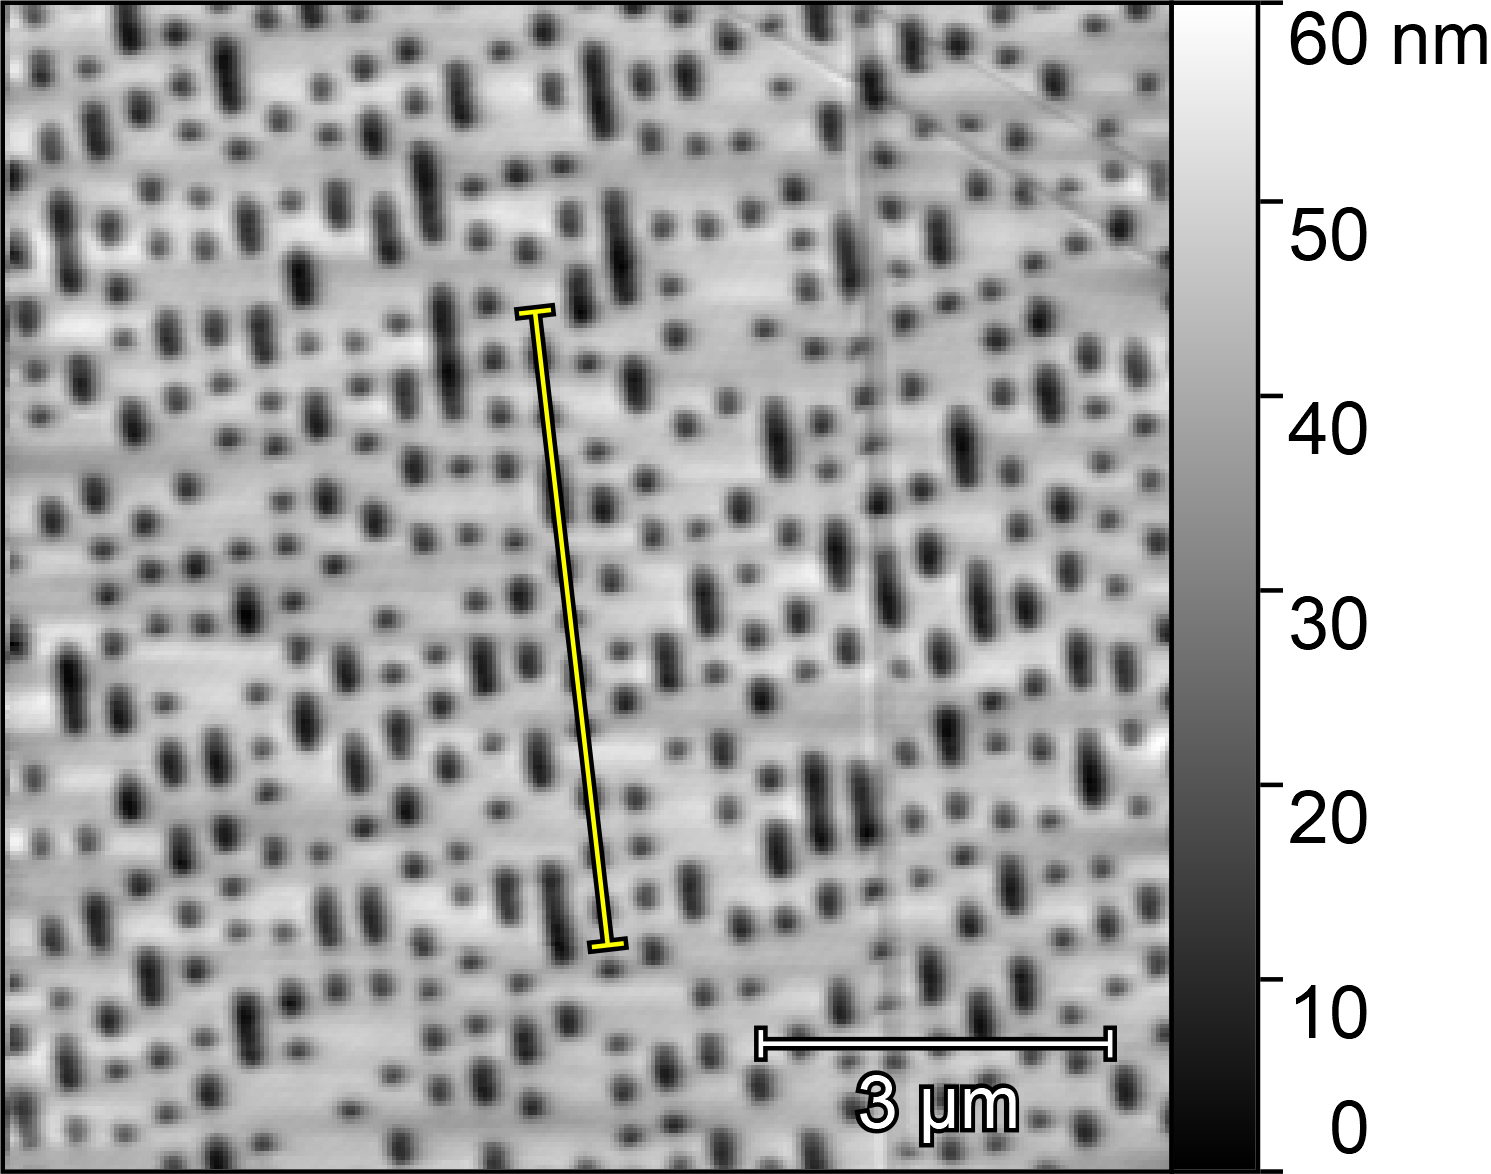
\includegraphics[width=10cm]{hddvd_topo.png}
    \caption{Topografia płyty HD DVD}
    \label{fig:hddvd_topo}
  \end{figure}

  \begin{figure}[H]
    \centering
    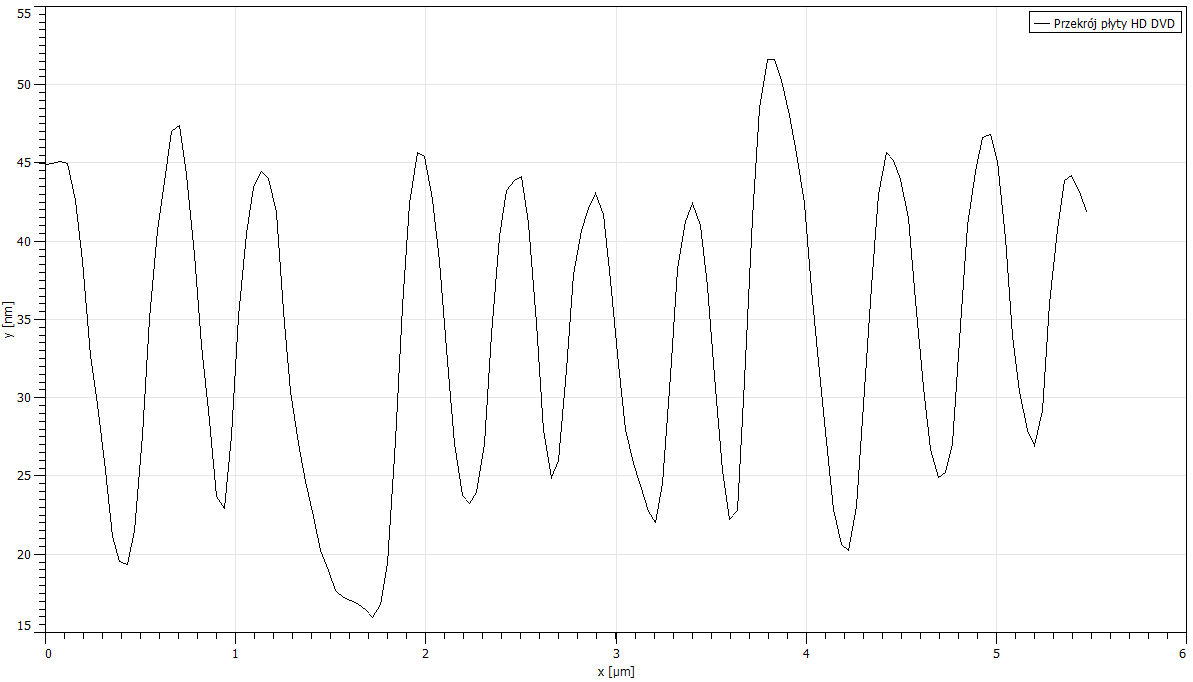
\includegraphics[width=10cm]{hddvd_przekroj.png}
    \caption{Przekrój płyty HD DVD}
    \label{fig:hddvd_przekroj}
  \end{figure}

  Po obcięciu obrazu tak aby powierzchnia była identyczna do powierzchni obrazu
  płyty DVD, możemy policzyc ilość rowków na płycie HD DVD.

  \begin{figure}[H]
    \centering
    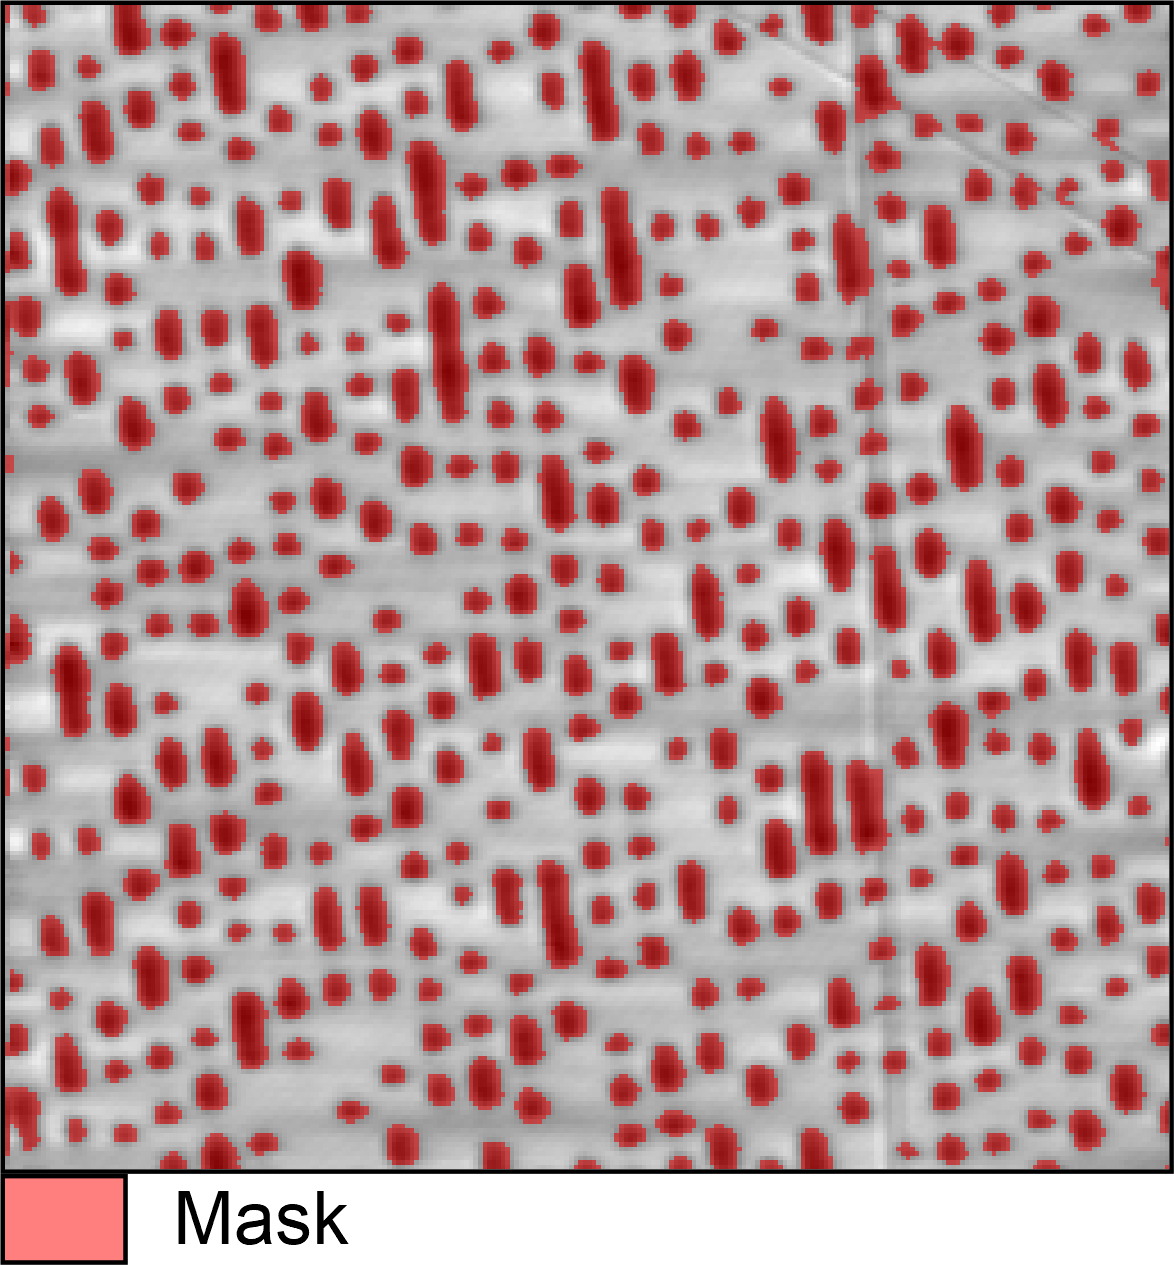
\includegraphics[width=10cm]{hddvd_grains.png}
    \caption{Obraz po zaznaczeniu rowków dla płyty HD DVD}
    \label{fig:hddvd_grains}
  \end{figure}

  \begin{table}[H]
    \centering
    \begin{adjustbox}{max width = .5\textwidth}
      \begin{tabular}{cc}
        \toprule
        \textbf{Nośnik}   & \textbf{Liczba rowków} \\
        \midrule
        DVD               & 90                     \\
        HD DVD            & 280                    \\
        \midrule
        \textbf{Stosunek} & 3.11                   \\
        \bottomrule
      \end{tabular}
    \end{adjustbox}
    \caption{Liczba rowków na obu płytach}
    \label{tab:grain_num}
  \end{table}

  \section{Wnioski}
  Na otrzymanych obrazach topografii badanych próbek zauważyc możemy wiele szumów
  czy błędów oraz zabrudzeń. Wynika to z niskiej klasy mikroskopu oraz niewielkiej
  ilości czasu na przygotowanie próbek oraz kalibrację urządzenia i wykonanie
  pomiarów.
  
  Obliczony stosunek pojemności płyt jest zbliżony do rzeczywistego
  (\( \approx 3,19 \))

  \clearpage
  \begin{thebibliography}{9}
    \addcontentsline{toc}{section}{Bibliografia}
    
    \bibitem{binnig}
    Binnig, G.; Quate, C. F.; Gerber, Ch\\
    \textit{Atomic Force Microscope}\\
    Physical Review Letters. 56 (9): 930–933. 

    \bibitem{feynman}
    Feynman Richard P.; Leighton Robert B.; Matthew Sands\\
    \textit{Feynmana wykłady z fizyki Tom I}
  \end{thebibliography}
\end{document}